%% Author: Julie Hoffer
%% Subject: Survival Analysis


The following questions refer to this graph:

\centerline{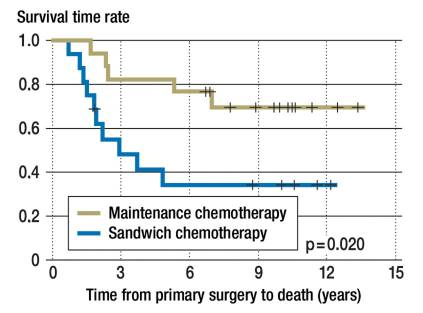
\includegraphics[width=3.2in]{final112-survival.jpg}}

\begin{enumerate}
\item What is the median survival time for children and adolescents receiving sandwich chemotherapy?

\answerSpace{1cm}

\begin{AnswerText}
3 years
\end{AnswerText}

\item What is the median survival time for children and adolescents receiving maintenance chemotherapy?

\answerSpace{1cm}

\begin{AnswerText}
Cannot be determined
\end{AnswerText}

\item What is the 10 year survival rate for chemotherapy and sandwich therapy?

\answerSpace{1cm}

\begin{AnswerText}
Chemotherapy:  70\%

Sandwich Therapy:  36 - 37\%
\end{AnswerText}

\item From this survival curve, which treatment seems to offer children and adolescents with medulloblastoma the best option.

\answerSpace{1cm}

\begin{AnswerText}
Chemotherapy
\end{AnswerText}

\item The small + signs indicate when a subject is lost to follow up.  Why doesn't the curve height change when there is such an event?

\answerSpace{2cm}

\begin{AnswerText}
Loss to follow up doesn't provide evidence of mortality, so there is no reason for the curve to change height.
\end{AnswerText}

\end{enumerate}
